\chapter{Løsning}
\lhead{Løsning}

\section{Krav}
For å se kravlisten av prosjektet viser jeg til kapittel \ref{kravliste1} for å se hvilke krav som ble utarbeidet i samarbeid med bedriften, og kapittel \ref{kravliste2} for å se den mer detaljerte liste over alle  featurelist fremgangsmåten som ble fulgt.

Ut av kravene ble et workflow utarbeidet, dette skal ta seg av bestillingsprosessen utarbeidet.

\subsubsection{Workflow}
\begin{steps}{Steg}
\step \textbf{Forside}\\Man starter med å se på forsiden av nettsiden. Denne skal inneholde generell informasjon om bedriften, litt om hvordan leien fungerer, priser, vilkår osv. Utover dette skal det her være 2 muligheter for brukeren å gå videre i reservasjonsprosessen:\\
\textbf{Søke på Dato} Her skal systemet finne ut hvilke biler som er ledige i en leieperiode, og returnere disse. \\
\textbf{Se Biler} Man kan se alle bilene innenfor en gitt kategori, eller alle biler i systemet.

\step \textbf{Liste over biler}\\Uavhengig av fremgangsmåten brukeren har valgt, vil man nå presenteres med en liste over biler. Listen inneholder generell informasjon om hver av bilene, samt bilde og døgnpris i leien.\\
Utifra denne listen velger brukeren å gå videre på en av bilene.

\step \textbf{Spesifikk bil}\\Nå befinner brukeren seg på siden til den bestemte bilen. Her skal informasjon om bilen og eventuelle bilder presenteres.
Dersom brukeren ikke søkte på dato i Steg 1, må det her sjekkes når bilen er ledig for utleie. Dette skal visualiseres i form av en kalender.\\
Videre skal brukeren fylle inn dato i leieperioden (Dersom man søker på Dato i Steg 1, skal dette bli fylt inn automatisk), så gå videre.

\step \textbf{Kontakt Informasjon}\\Det siste steget av reservasjonsprosessen. Her skal brukeren fylle inn kontakt informasjon, og kunne se informasjon om reservasjonen og den valgte bil.\\
Når informasjonen er fylt inn trykker brukeren på Fullfør Bestilling, som skal videreføre til en bekreftelses side om hele bestillingen. Nå skal også en epost bli sendt til brukeren som inneholder informasjon om bestillingen.

\step \textbf{Last ned informasjon som PDF (Valgfritt)}\\Brukeren skal ha mulighet til å laste ned ordre bekreftelse som PDF 

\end{steps}




\section{Designspesifikasjoner}
Det ble i hovedsak satt 2 krav til design for nettsiden. Den skal skalere godt mellom skjermstørrelser, og den skal være så oversiktlig og lett å bruke som mulig.

\subparagraph*{Skalering}
For å oppnå god skalering mellom skjermstørrelser ble rammeverket Bootstrap benyttet. Ved å bruke Bootstrap vil man jobbe med Grid systemet som lar deg konfigurerer hvordan den skal takle plassering av elementer på små og store skjermer. 

\subparagraph*{Oversiktlig}
Det er litt vanskeligere å tilfredsstille kravet om at det skal være oversiktlig da dette er noe mer subjektivt, og meninger vil variere fra bruker til bruker. Men det har blitt utarbeidet en løsning med så lite støy som mulig. Dvs. alt av innhold på nettsiden skulle ha en grunn til å være der. 
%Sette Workflow her?

\newpage
\section{Resultat}

\subsection{Forsiden}
På forsiden av nettsiden (Figur \ref{fig:rv_frontpage}) finner man de to elementene for å finne frem til en bil for utleie. Her har man valget av å enten søke på dato i leieperioden, eller man kan få en liste over bilene. Ved å søke på dato har man også valget om å spesifisere hvilke biltyper som skal være med i søket. \\

Utover dette har vi ytterligere informasjon i form av seksjoner, her finner man vilkår, informasjon, kontakt informasjon og om oss.

 \begin{figure}[htbp]
	\centering
		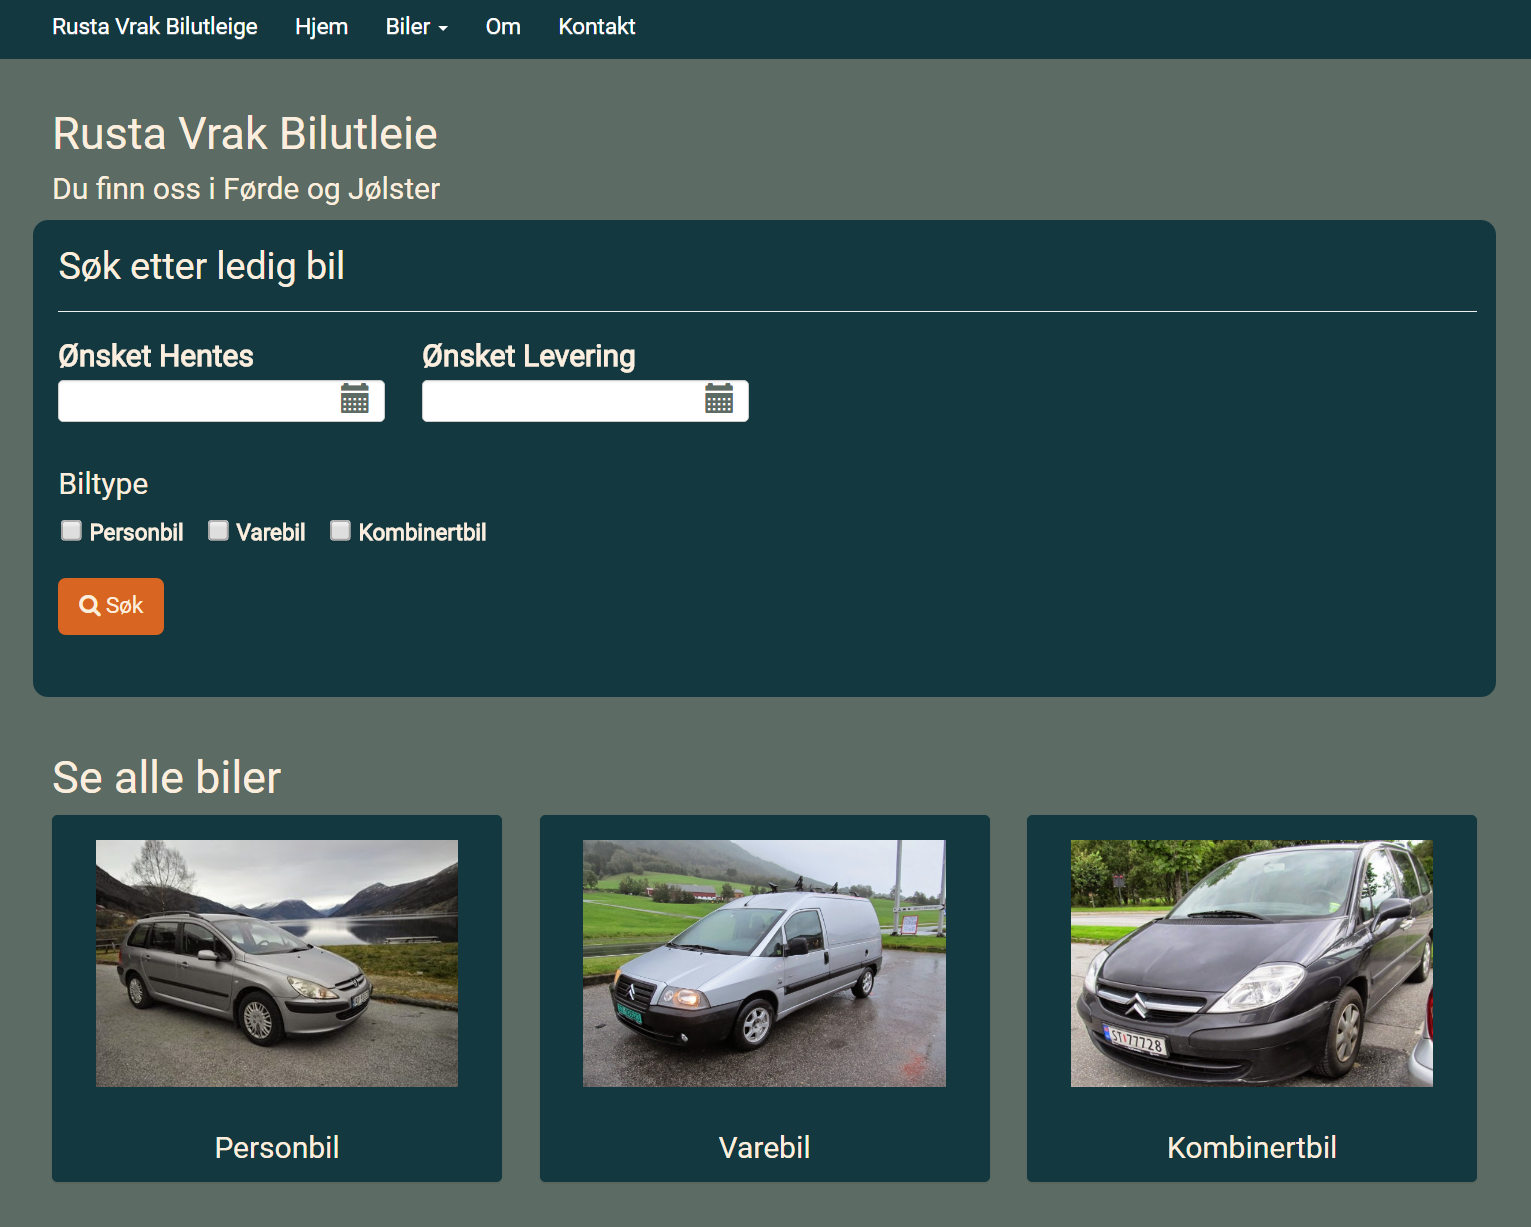
\includegraphics[scale=0.4]{Bilder/rv_frontpage.png}
	\caption[Forsiden til Nettsiden]{Forsiden til nettsiden. Her kan man se de to valgene brukeren kan ta for å finne frem til bil. Enten vha. Søk etter ledig bil i form av leieperiode, eller liste over alle biler. } %\ref{fig:iterative}
	\label{fig:rv_frontpage}
\end{figure}


\subsection{Liste over Biler}
Denne siden viser alle biler som ble søkt fra forsiden, se figur \ref{fig:rv_carlist}. Dersom et det ble gjort et søk på dato, vil alle bilene i listen være ledig i den gitte periode. Hver bil har et hovedbilde, som kan forstørres ved å klikke på bildet, og det blir oppgitt informasjon om hver bil som type girkasse, drivstoff, antall seter, diverse tilbehør og leiepris. 

 \begin{figure}[htbp]
	\centering
		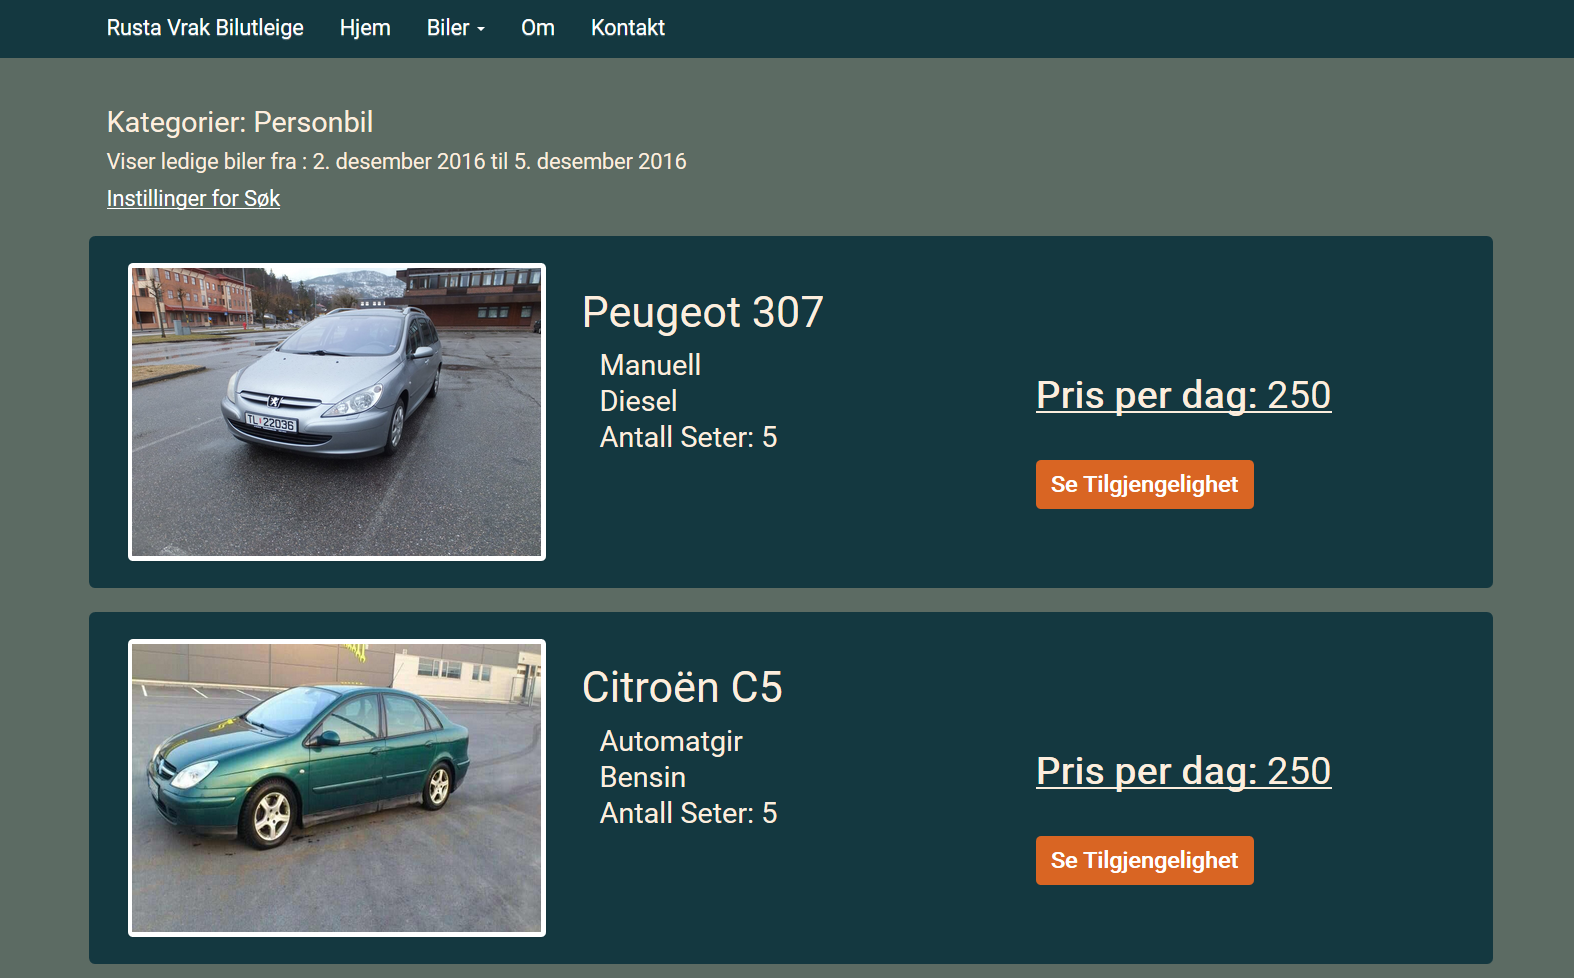
\includegraphics[scale=0.4]{Bilder/rv_carlist.png}
	\caption[Liste over Biler]{En liste over alle biler fra det oppgitte søk. Hver bil viser generell informasjon og har en knapp for å gå videre til den spesifikke bilen. } %\ref{fig:iterative}
	\label{fig:rv_carlist}
\end{figure}

Denne listen kan filtreres videre ved å trykke på «Innstillinger for Søk». Se figur \ref{fig:rv_carlist_filter} Her kan man velge å spesifisere ytterligere hvilke egenskaper en bil skal ha, dette inkl. valg av til biltyper, type girkasse, drivstofftype og antall seter. Ved å trykke på filter knappen vil serveren generere en ny liste som oppfyller de oppgitte kravene i instillingene.

 \begin{figure}[htbp]
	\centering
		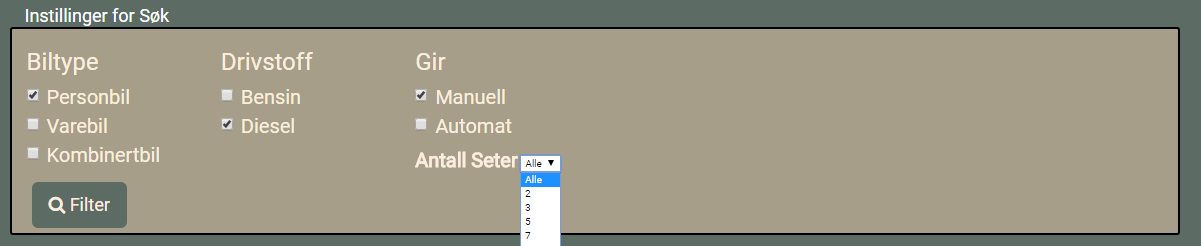
\includegraphics[scale=0.5]{Bilder/rv_carlist_filter.png}
	\caption[Instillinger for Søk]{En filtreringsmeny for å kunne spesifisere ytterligere hvilke biler som skal bli oppgitt i listen.} %\ref{fig:iterative}
	\label{fig:rv_carlist_filter}
\end{figure}



\subsection{Individuelle Biler}
Siden som fremstiller de individuelle bilene er identisk for alle biler, og viser bilde (og eventuelt galleri dersom flere bilder er oppgitt), informasjon om bilen, input områder for å foreta en reservasjon og en kalender som fremstiller når bilen er ledig for utleie.

 \begin{figure}[htbp]
	\centering
		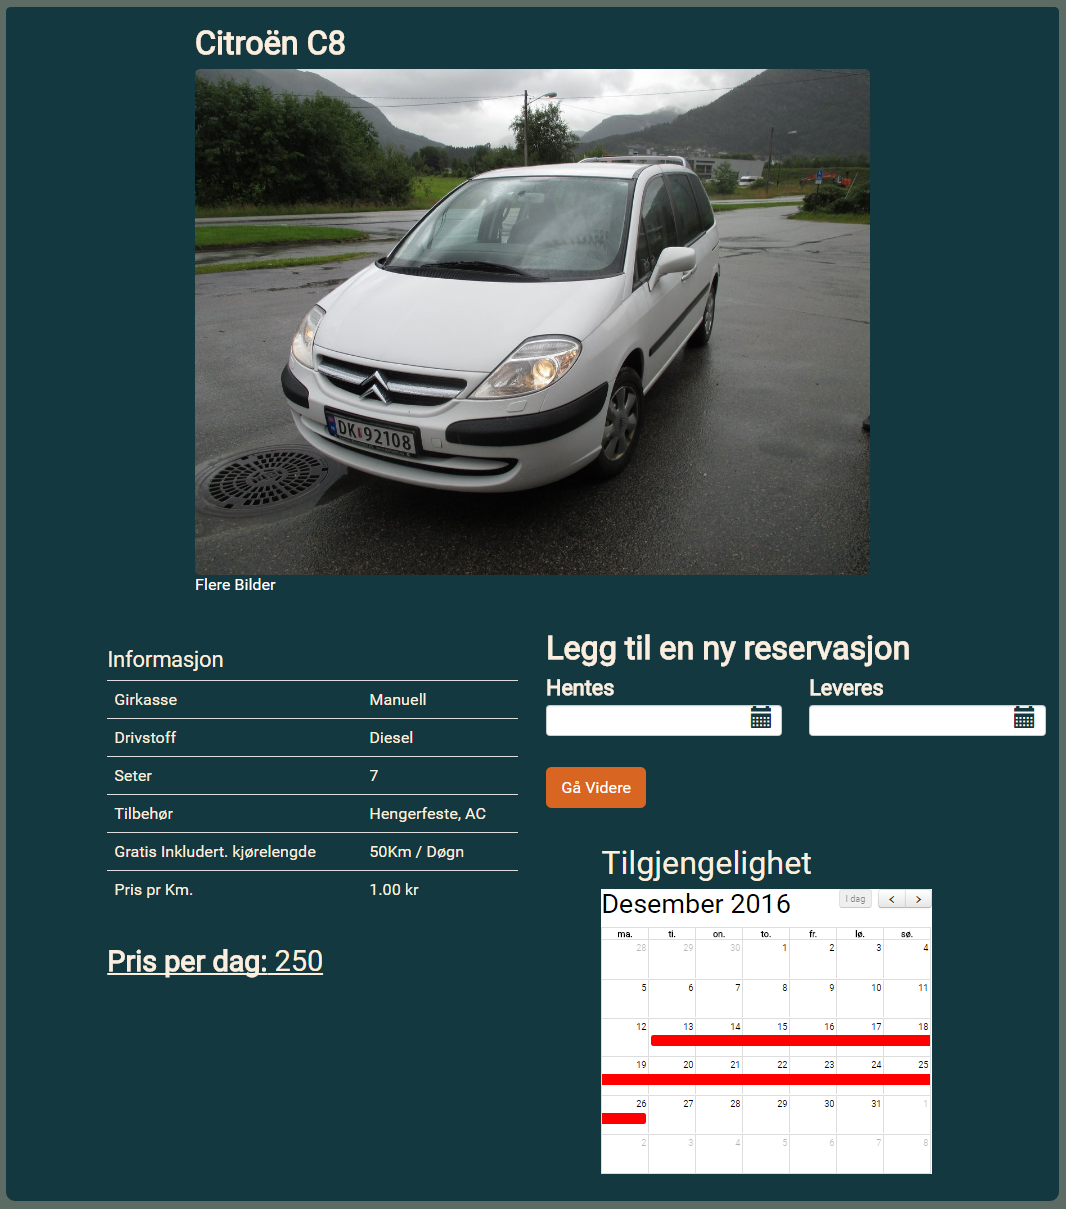
\includegraphics[scale=0.3]{Bilder/rv_individualcar.png}
	\caption[Individuelle Biler]{ Siden til de individuelle bilene. Her vil man få oppgitt generell informasjon om bilen, bilder, funksjonalitet for å reservere bilen og en kalender som visuelt fremstiller når bilen er ledig for utleie.} %\ref{fig:iterative}
	\label{fig:rv_individualcar}
\end{figure}

Når det opprettes en ny reservasjon, vil systemet først sjekke om den oppgitte perioden er en gyldig, de sjekker som blir gjort er som følger:
\begin{enumerate}
\item Hente dato er satt før leveringsdato.
\item Leieperioden er større enn 0 og mindre enn 31 (maks leieperiode man kan opprette på egenhånd er 30 dager.
\item Leieperioden ikke satt tilbake i tid.
\item Leieperioden for den spesifikke bilen er ledig. Jeg viser til vedlegg D for å se koden.
\end{enumerate}

Dersom alle kravene er oppfylt, vil brukeren omdirigeres videre til neste steg i reservasjons prosessen.

%\begin{figure}[htbp]
%	\centering
%		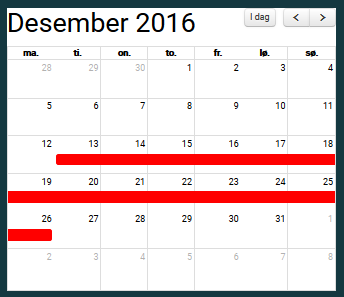
\includegraphics[scale=0.5]{Bilder/rv_dateavailable.png}
%	\caption[Utleiepris Diagram]{Oversikt over rabatt som tilføres i forhold til hvor lenge en bil blir utleid. } %\ref{fig:iterative}
%	\label{fig:rv_dateavailable}
%\end{figure}



\subsection{Kontaktskjema}
Etter brukeren har valgt en bil, og funnet en ledig periode for utleie må det til slutt fylles ut et kontaktskjema (Figur \ref{fig:rv_customercontact}). Her må det fylles ut enkel informasjon om kunden: epost, fornavn, etternavn og telefonnummer. Man har også et valgfritt tekstområde for eventuell ekstra informasjon man ønsker å oppgi, eller om det skulle være noen spesielle omstendigheter ved leien.
\\
I tillegg har får man oppgitt informasjon om valg leieperiode, pris, og den valgte bilen. 

 \begin{figure}[htbp]
	\centering
		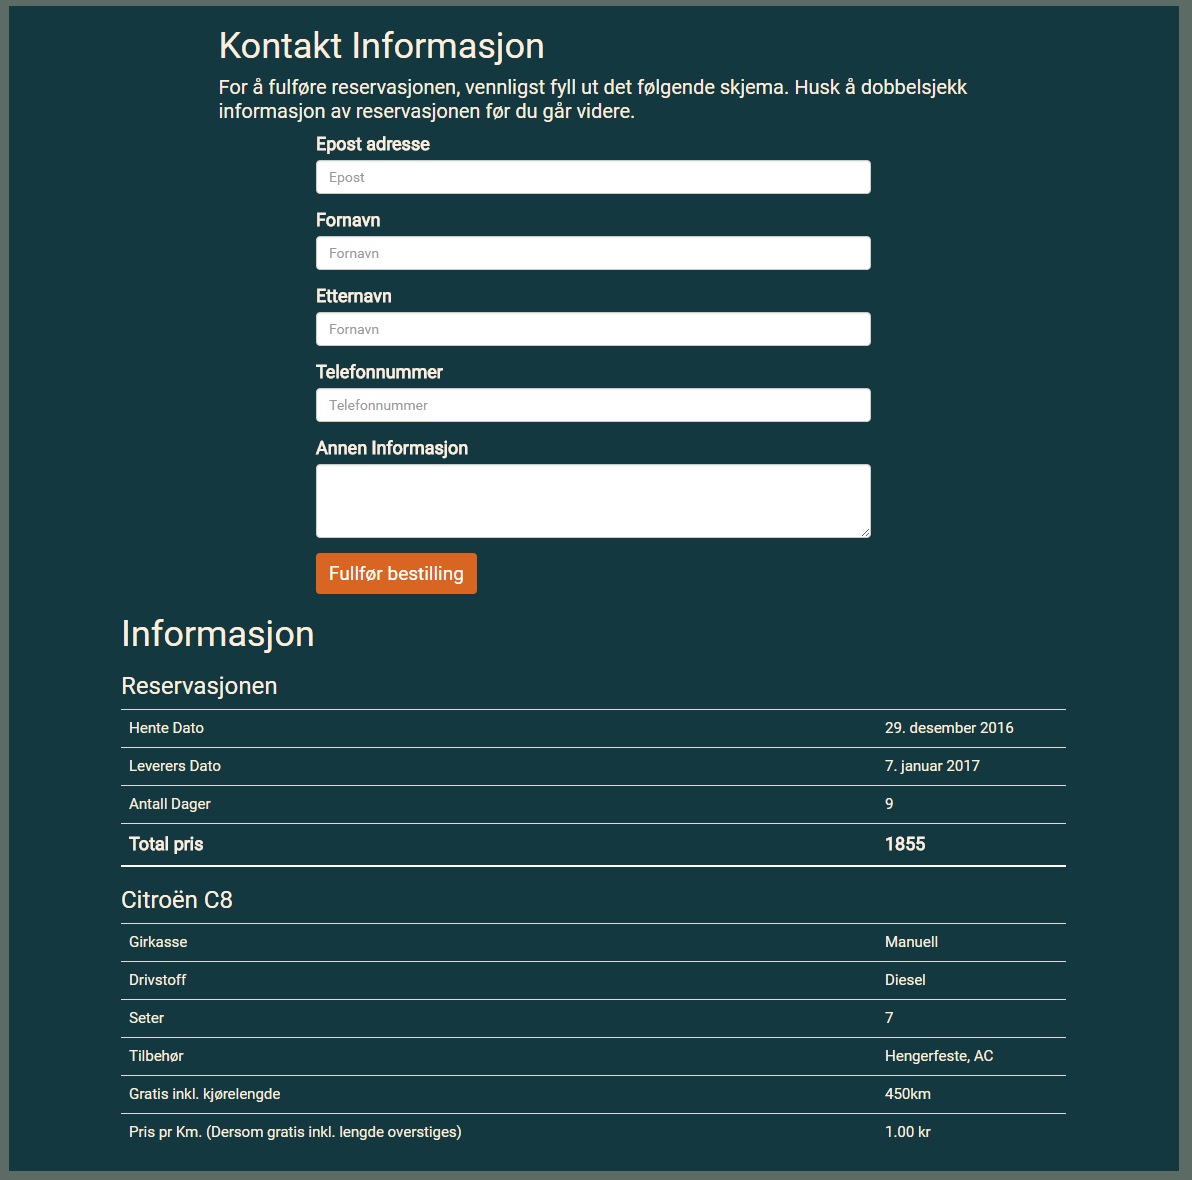
\includegraphics[scale=0.5]{Bilder/rv_customercontact.png}
	\caption[Kontaktskjema]{Det siste steget i bestillingsprosessen. Her må man fylle inn kontaktskjemaet. Man har også her muligheten til å se alle detaljer omgående reservasjonen.} %\ref{fig:iterative}
	\label{fig:rv_customercontact}
\end{figure}

\subsection{Bekreftelse}
Når bestillingen er vellykket og er blitt lagret til databasen, blir brukeren videresendt til en bekreftelses side (Figur \ref{fig:rv_customercontact}). Her finner man all informasjon om reservasjonen, og man har et valg om å laste ned en PDF som inneholder samme informasjon (Vedlegg A). Utover dette blir det også sendt en epost til brukeren, som også inneholder all informasjon om reservasjonen.



 \begin{figure}[htbp]
	\centering
		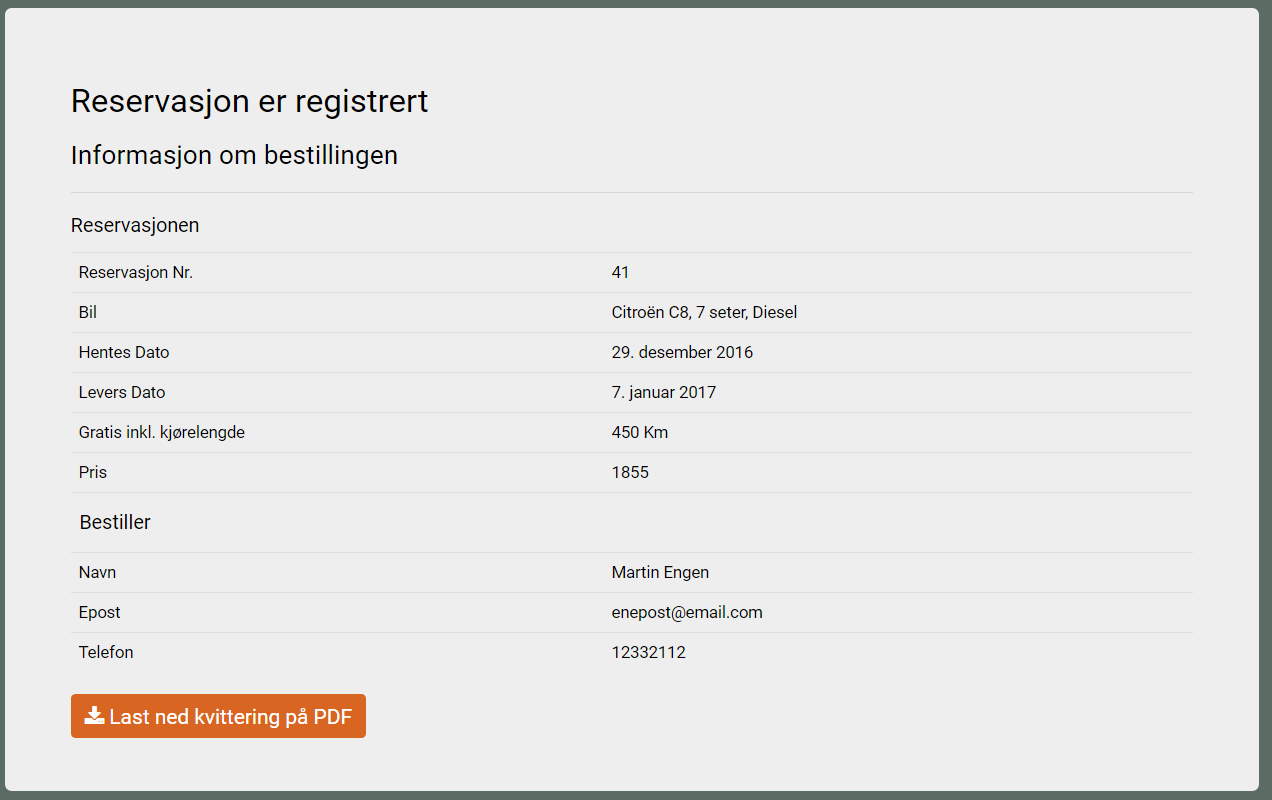
\includegraphics[scale=0.5]{Bilder/rv_receipt.png}
	\caption[Ordre Bekreftelse]{Det siste steget i bestillingsprosessen. Her må man fylle inn kontaktskjemaet. Man har også her muligheten til å se alle detaljer omgående reservasjonen.} %\ref{fig:iterative}
	\label{fig:rv_customercontact}
\end{figure}



\clearpage
\section{Administrasjon}
Administrasjonssiden skal hovedsakelig benyttes av bedriften for å kunne holde et styr over sine biler og bestillinger. På figur \ref{fig:admin_front} kan man se et skjermbilde av forsiden av admin siden. Denne admin siden blir generert av Django og reflekterer de konfigurasjonene som blir gjort i koden. Her velges bl.a. hvilke tabeller som er interessante å ha i admin siden, hvilke elementer som skal ligge i listen, hva som er relevant i søke funksjoner osv. Her har man også muligheten til å opprette nye admin kontoer og velge hvilke rettigheter de skal kunne ha på nettsiden.

 \begin{figure}[htbp]
	\centering
		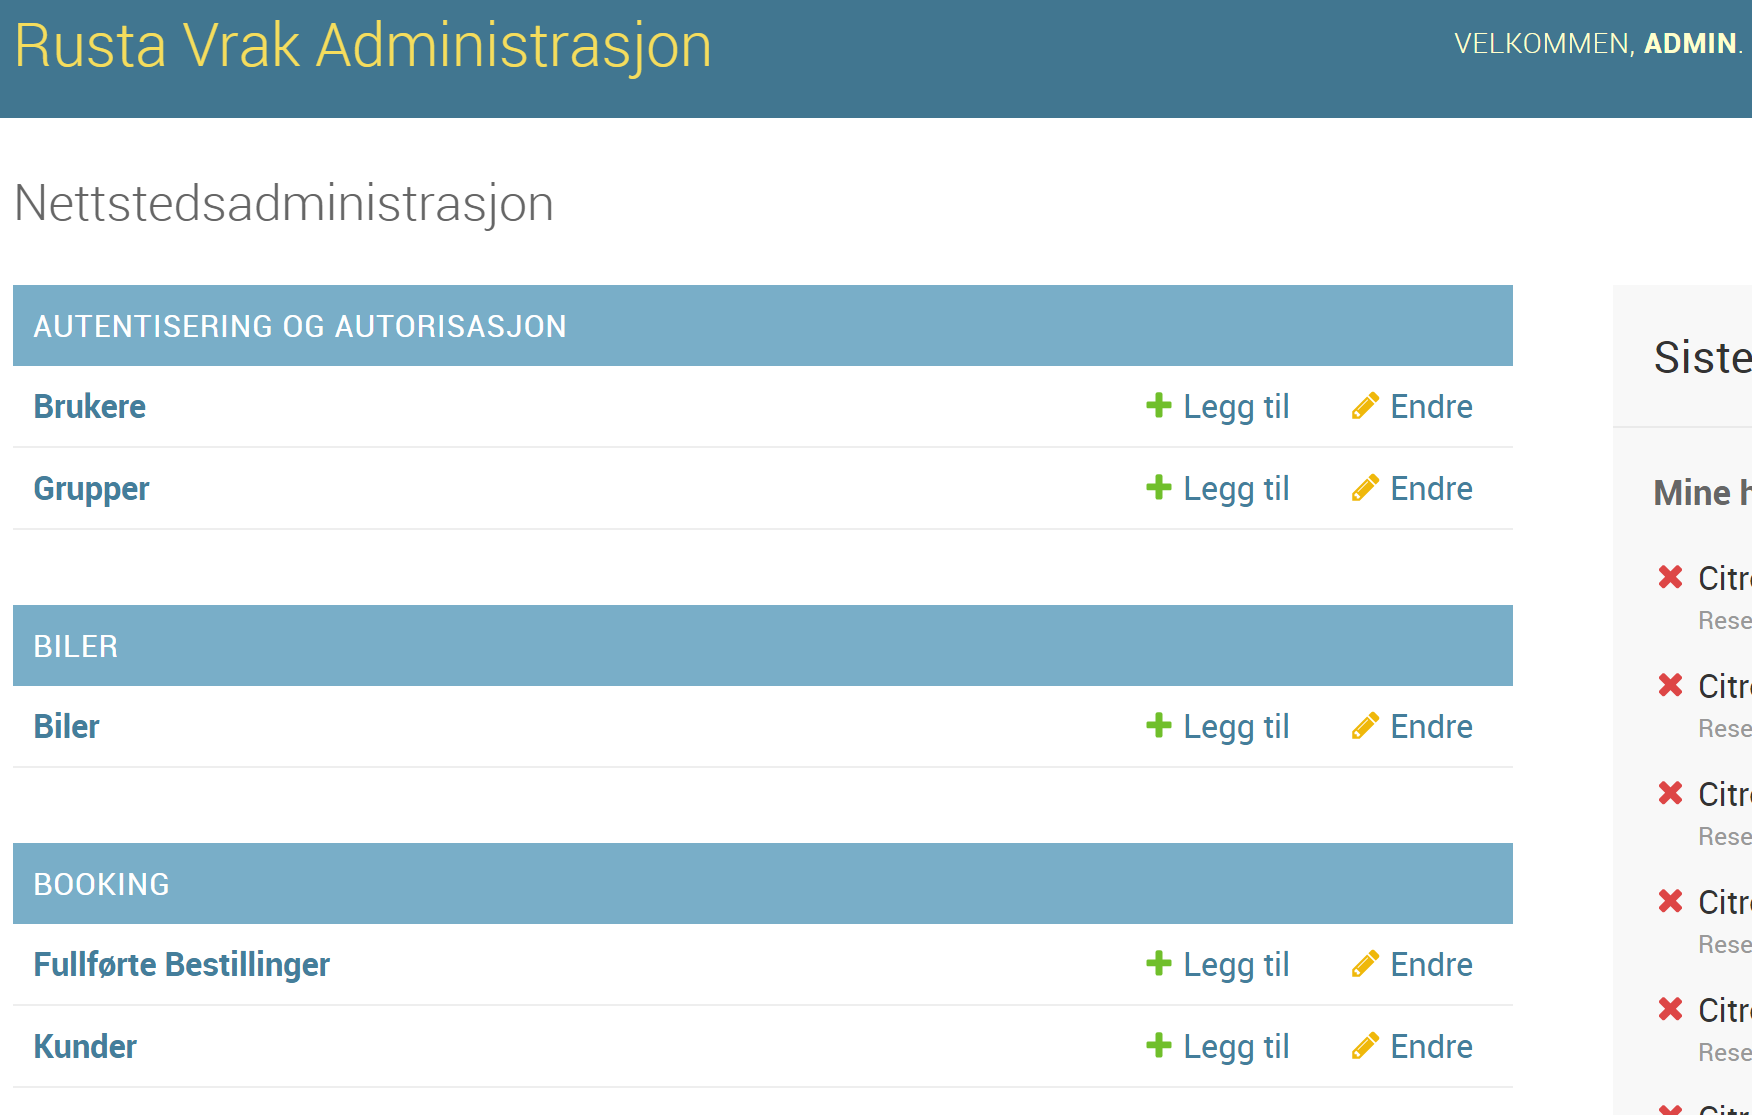
\includegraphics[scale=0.3]{Bilder/admin_forside.png}
	\caption[Forside i Administrasjons Side]{Hvordan administrasjonssiden ser ut. Denne har blitt generert og konfigurert med web-applikasjons rammerverket Django. } %\ref{fig:iterative}
	\label{fig:admin_front}
\end{figure}
\newpage
\subsection{Reservasjoner i Administrasjonsside}
På figur \ref{fig:admin_list} kan man se listen over alle ferdig reservasjoner. Her kan man se informasjon om kunden, hvilken bil som er reservert, bestillings, hente og leveringsdato, og den totale prisen for reservasjonen. \\
For å kunne filtrere ut spesifikke reservasjonen kan man bruke søke funksjonen. Denne godtar søk på skiltnummer, bilmerke og modell, kundens etternavn og epost. Søket blir gjort å en såkalt «Contains» metode, som betyr at dersom man f.eks. gjør et søk på ‘TV’, vil reservasjonen med en bil med skiltnummer ‘TV65282’ bli med i resultatet.

 \begin{figure}[htbp]
	\centering
		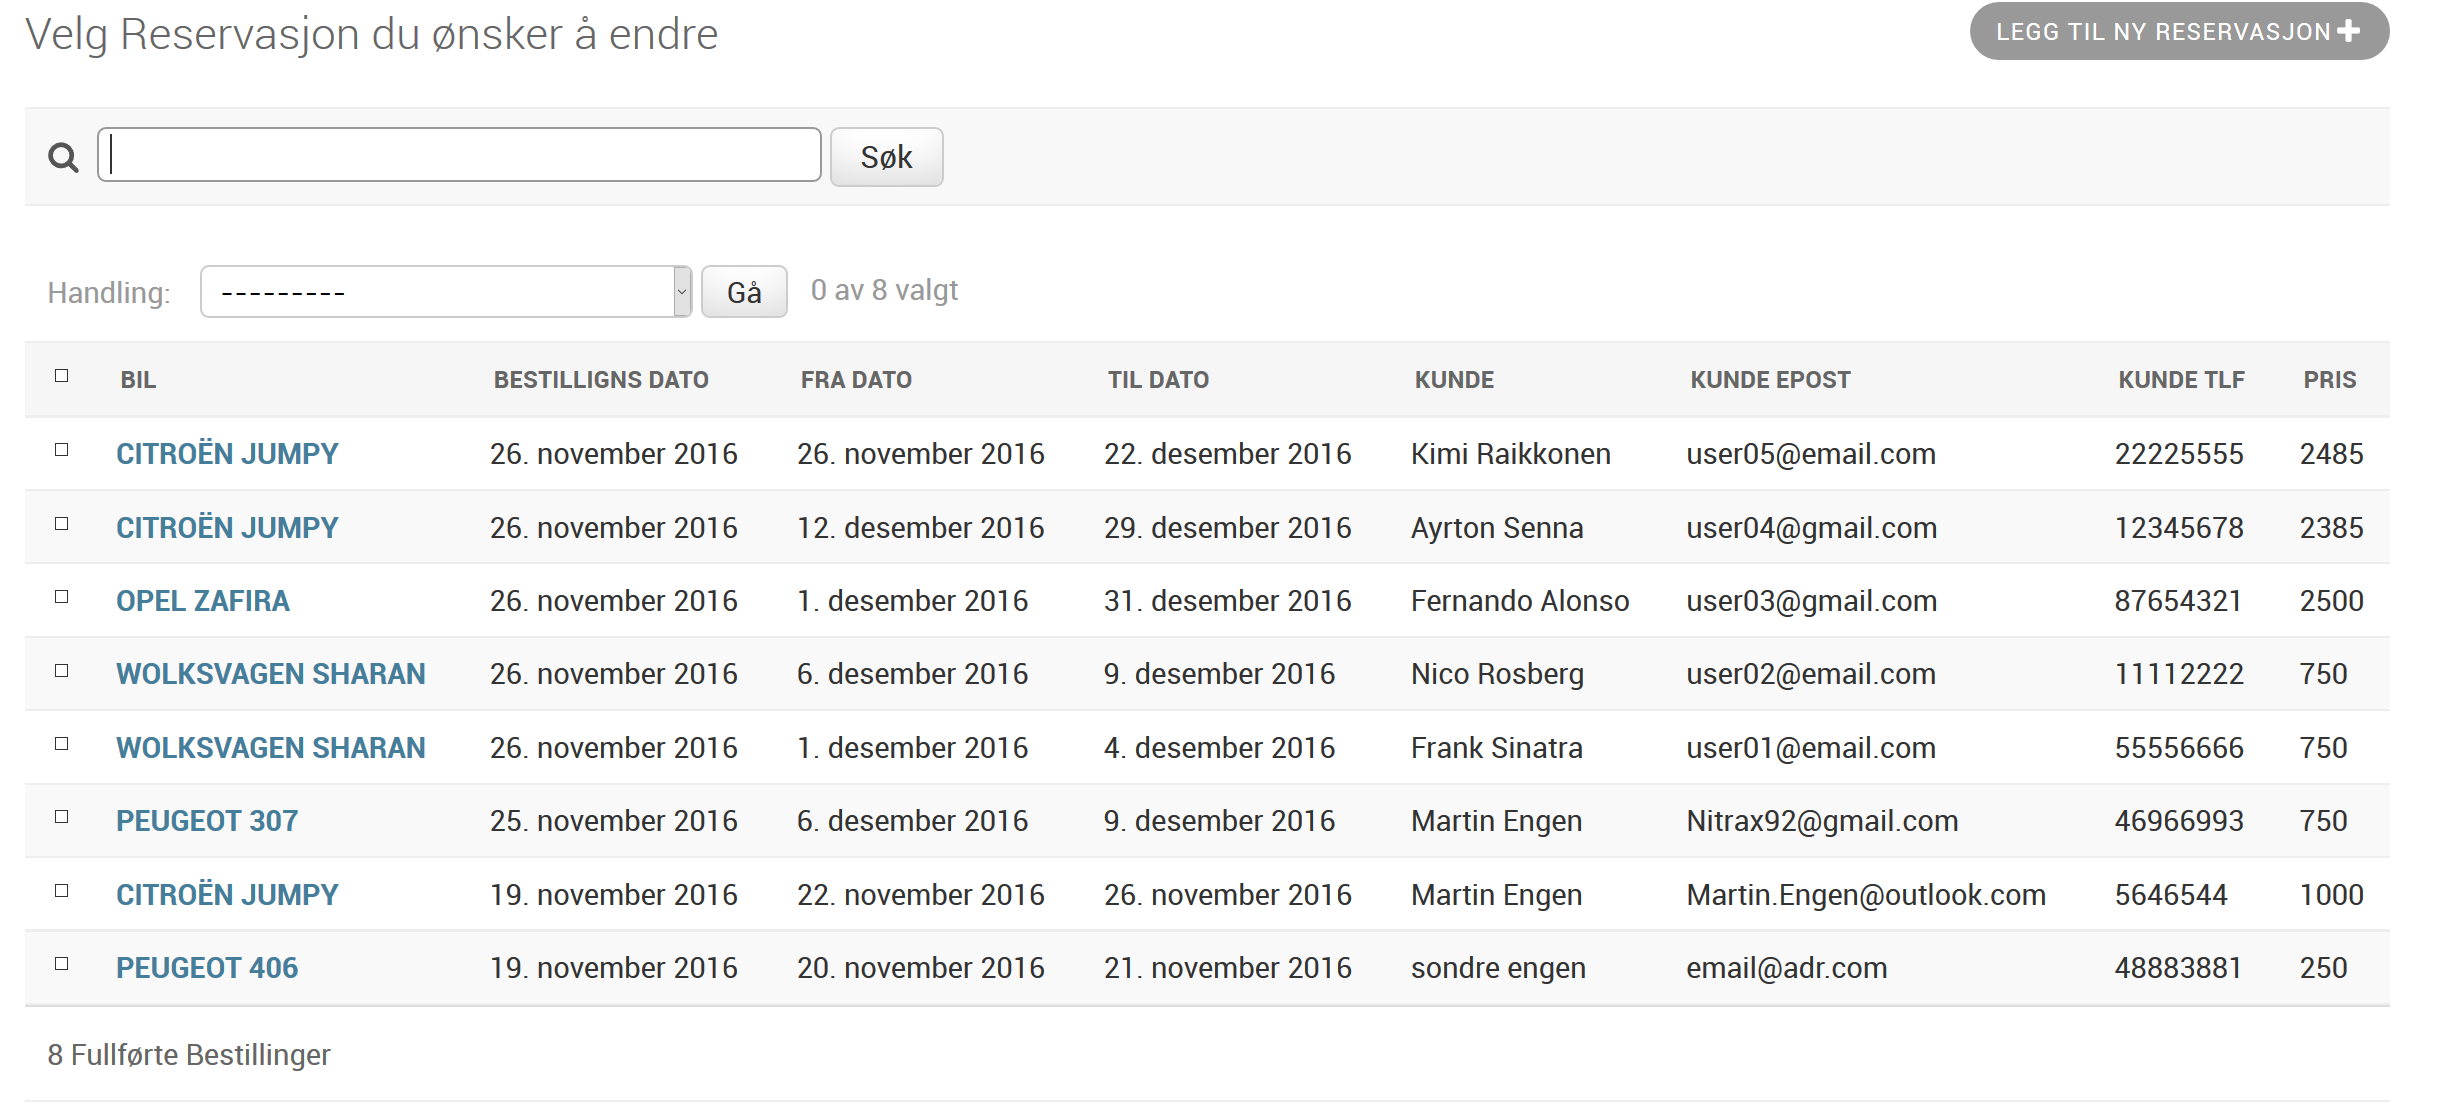
\includegraphics[width=16cm, keepaspectratio]{Bilder/admin_liste2.png}
	\caption[Administrasjonsside - Oversikt over reservasjoner]{Liste over alle reservasjoner registert på nettsiden. } %\ref{fig:iterative}
	\label{fig:admin_list}
\end{figure}





\subsection*{Legge til ny reservasjon}




\begin{figure}[h!]
\begin{flushright}
\begin{minipage}{0.5\textwidth}
\begin{center}
    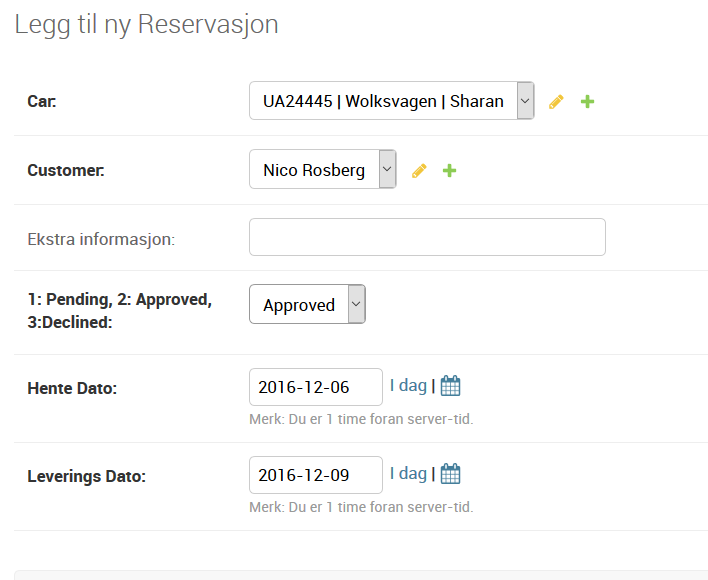
\includegraphics[width=1\textwidth]{Bilder/admin_ny_reservasjon.png}
    \caption[Ny reservasjon fra administrasjonsside]{Hvordan man legger inn en ny reservasjon direkte fra administrasjonssiden.}
    \label{fig:admin_new_res}
\end{center}
\end{minipage}
\end{flushright}
\end{figure}


%
\vspace{-7cm}
%
\begin{flushleft}
\begin{minipage}{0.4\textwidth}

%
%
Dersom en kunde ikke ønsker å reservere gjennom nettsiden, kan ansatte også gjøre dette manuelt gjennom administrasjons siden. Dette er en enkel prosess, man velger å legge til en ny reservasjon, fyller ut vinduet (Se Figur \ref{fig:admin_new_res}) og lagrer dette.

\end{minipage}
\end{flushleft}

\newpage


\section{Database}
Dette prosjektet benytter Django, og dermed vil dette rammeverket ta hånd om mye av arbeidet mot databasen. Django kommer utstyrt med en ORM (Object Relational Mapper), som håndterer overgangen fra Python klasser til MySQL tabeller.
 
Figur \ref{fig:tables} viser de tabellene som er direkte knyttet til biler, kunder og reservasjoner på nettsiden. Her har det blitt brukt et utviklet et enkelt system, da det ikke var behov for noe mer utbredt. En mulig forbedring ville vært å splitte Car tabellen opp i flere små tabeller, men per i dag trenger man all informasjon om bilen hver gang den hentes fra databasen, så en refaktorering har ikke vært en prioritet. 

For å se et komplett bilde av alle tabeller i databasen viser jeg til vedlegg C.

 \begin{figure}[htbp]
	\centering
		\includegraphics[scale=0.7]{Bilder/db01.png}
	\caption[Tabellene i Database]{Tabellene i databasen direkte knyttet til bilene, kundene og reservasjonene. } %\ref{fig:iterative}
	\label{fig:tables}
\end{figure}


\newpage
\section{Priser og Rabatt}
Rusta Vrak Bilutleige ønsker at når en kunde først skal leie en bil, skal det være så lenge som mulig for å slippe å hente og levere biler mer enn nødvendig. Derfor vil bedriften gi kunder gode rabatter som øker i forhold til lengde på leieperiode. Leieprisen av de aller fleste bilene ligger på 250kr pr. døgn, og bedriften tilbyr utleie på disse bilene i 30 dager for kun 2500kr. Dette tilsvarer en prisreduksjon på 66.6\%. For å kunne implementere et liknende system på nettsiden ble det laget en rekke løsningsforslag i Excel, dette finner man vedlagt i vedlegg Y

\subsection*{Valgte Løsning}
Den valgte løsningen går ut på å gi kunden 17.5\% ekstra avslag hver 5. dag i leieperioden. Se tabell \ref{table:percent} for en oversikt over hvordan pris avslaget stiger. Figur \ref{fig:price_reduction} viser hvordan prisantydningen blir på biler som har en døgnpris på 250kr. Dette vil kunne bidra til at en kunde leier litt ekstra kun for å få ekstra avslag på prisen. Koden bak den implementerte priskalkuatoren finner man i vedlegg D.

\begin{table}[htbp]
\centering
\caption{Rabatt man oppnår ved leieperioder}
\label{table:percent}
\begin{tabular}{|l|l|l|l|l|l|l|l|l}
\cline{1-8}
Antall Dager & 0-4   & 5-9    & 10-14     & 15-19    & 20-24    & 25-29    & 30      &  \\ \cline{1-8}
Rabatt       & 0\% & 17.5\% & 31.9375\% & 43.849\% & 53.675\% & 61.782\% & 66.66\% &  \\ \cline{1-8}
\end{tabular}
\end{table}



 \begin{figure}[htbp]
	\centering
		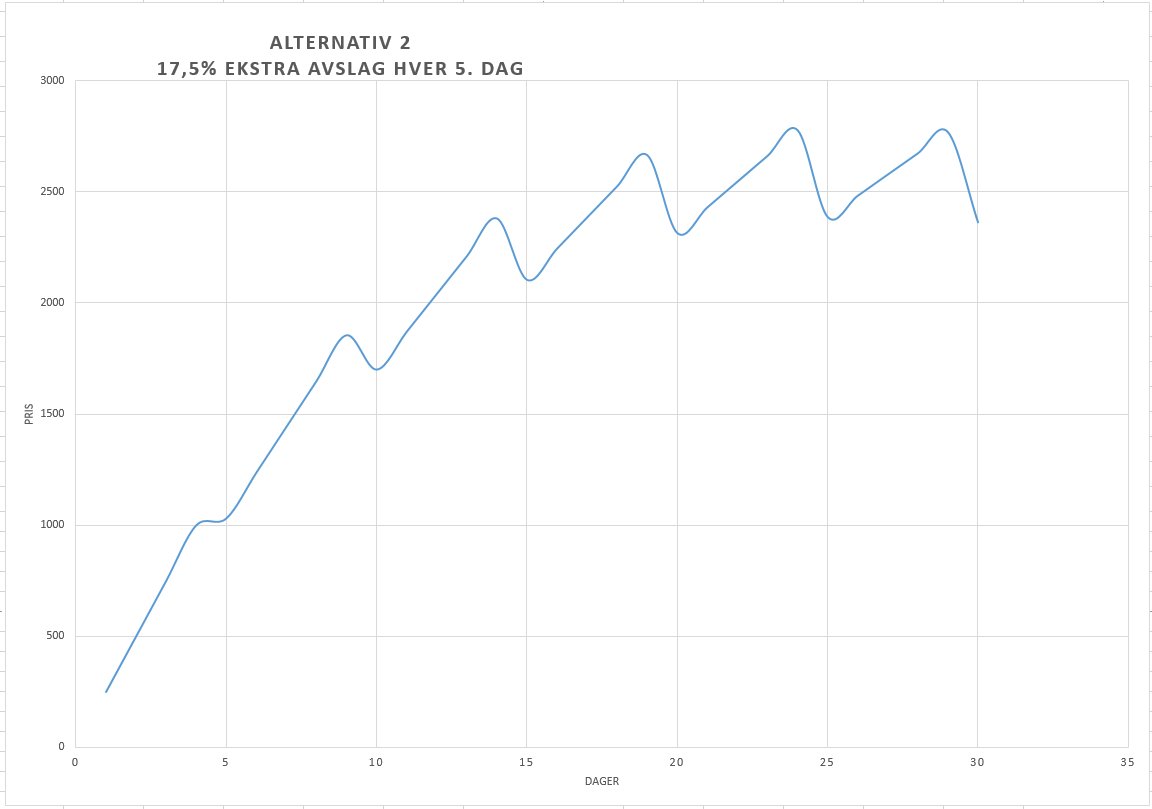
\includegraphics[scale=0.5]{Bilder/avslag2.png}
	\caption[Utleiepris Diagram]{Oversikt over rabatt som tilføres i forhold til hvor lenge en bil blir utleid. } %\ref{fig:iterative}
	\label{fig:price_reduction}
\end{figure}




\clearpage


\clearpage
\section{Testing og Validering}
Det har blitt benyttet en iterativ arbeidsmetode som beskrevet tidligere: Kapittel \ref{chap:method}. Denne metoden tilsier at testing skal og må foregå underveis i utviklingen i hver syklus. Dette har blitt gjennomført vha. Pythons logging bibliotek, Djangos debuggings modus og Djangos system check. 

\subsection{Django Debugging}
En av hovedegenskapene til debugginsmodus er at man vil få detaljerte error sider.  Dersom en appliaksjon kjører seg fast vil man få oppgitt en side med detaljert traceback, data om miljøet og eventuelle SQL query som blir utført i sammenheng med krasjet \cite{django:debug}. \\
Dersom man slår av debuggingsmodus vil applikasjonen redirigere til en standard error side (404, 400 etc.) ved feil.


\subsection{Django System Check}
Kommandoen ‘python manage.py check’ kjører en bred sjekk av hele systemet \citep{tests:django}. Denne vil gå grundig gjennom følgende deler av prosjektet:
\begin{description}
\item[Modeller.]Går gjennom alle database modeller og sjekker om modeller, og felter er som de skal være, og reflekterer tabellene i databasen.
\item[Admin.]Ser på alle egendefinert Admin funksjoner og oversiktstabeller. Først og fremst sjekker at alle tabeller inneholder virkelig data, og at de grunnleggende admin funksjoner (Legge til, slette, redigere) er funksjonelle.
\item[Kompatibilitet]Denne vil se at koden benytter Django’s anbefalte funksjoner, og vil gi advarsel dersom en nyere versjon av Django har forandringer, og hva som bør endres for å gjøre koden kompatibel med nyere django versjoner.
\item[Sikkerhet]Det blir utført en noe begrenset, men en såkalt ‘low-hanging-fruit’ sjekkliste. Dette er bl.a. en sjekk om at alle POST requests inneholder en Django spesifikk csrf token (Cross-site request forgery).
\item[Templates.]En gjennomgang av alle HTML som finnes til Templates mappene. Her blir det gjort en sjekk for å se om alle ‘tags’ \footnote{Man kan utføre logikk i HTML i form av Tags. Disse kan f.eks. bruke variable, enkle IF setninger og løkker. Tags blir evaluert når den blir generert av serveren før den sendes til brukeren i form av ren HTML \cite{django:tags}.} blir benyttet på korrekt måte.


\end{description}




\chapter{Diskusjon}

\lhead{Diskusjon}
% Domene
% Passe på ikke overlapp ved manuell registrering av bestillinger
%
\subsection*{Målet}
Hovedmålet til dette prosjektet var å utvikle en nettside for bedriften Rusta Vrak Bilutleige. Denne skulle fungerer som et bestillingsverktøy for kunder, og som et oversiktsverktøy for bedriften. Etter min mening har dette målet blitt møtt, og prosjektet er klart til å bli tatt i bruk.
Prosjektet skulle også publiseres, og dette har blitt gjennomført vha. Google App Engine. Jeg hadde tidligere erfaring med publisering på denne tjenesten, så denne prosessen var velkjent. Prosjektet er å finne på følgende URL: https://rusta-vrak.appspot.com/ 
\subsection*{Fremtidig Arbeid}
\paragraph*{Domene.}
Rusta Vrak har et eget domene, men det ligger fortsatt tilkoblet den gamle nettsiden. Dette må konfigureres for å kunne kjøre direkte til den nye nettsiden.

\paragraph*{Admin Reservasjoner.}
Det er fortsatt et problem som gjenstår å bli løst. I dag kan en admin registrere reservasjoner som overlapper med allerede eksisterende reservasjoner, uansett bil og kunde. Dette kommer av at admin systemet ikke er direkte knyttet til samme system brukere benytter for å legge inn nye reservasjoner, og dette burde bli tatt hånd om relativt snart for å unngå uheldige dobbelreservasjoner. 
Systemet fungerer godt når det legges inn nye reservasjoner fra perspektiv fra kunde, så derfor må ansatte som skal legge inn en ny reservasjon god kontroll på hvilke dato og biler som er ledige i en gitt periode.



\chapter{Konklusjon}
\lhead{Konklusjon}
Formålet med denne oppgaven var å utvikle en ny nettside for bedriften Rusta Vrak Bilutleige. Denne nettsiden skulle fungere som en alternativ bestillingsmetode for kunder, og hadde noen krav om at den skulle skalere godt over forskjellige skjermstørrelser, være lett og oversiktlig i bruk. Bedriften skulle også kunne benytte denne nettsiden som et oversiktsverktøy over sine biler, kunder og reservasjoner. Etter endt oppgaveperiode fyller nettsiden alle disse kravene og behovene, og produktet er klar til bruk.

Det finnes mange gode reserveringssider på internett, og det var nyttig å hente inspirasjon fra disse. Samtidig var det viktig å skreddersy nettsiden mot bedriftens formål, og dette har blitt gjennomført på en god måte.

%Målet med denne oppgaven var å utvikle en nettside for bedriften Rusta Vrak Bilutleige. Denne nettsiden skal kunne benyttes som både bestillingsverktøy for kunder, og som et oversiktsverktøy for bedriften. Etter endt prosjektperiode er nettsiden klar til bruk og alle kravene som ble satt i begynnelsen av perioden har blitt oppfylt. 